% Chapter 1

\chapter{Design and Implementation} % Main chapter title

\label{Chapter3} % For referencing the chapter elsewhere, use \ref{Chapter1} 

\lhead{Chapter 3. \emph{Design and Implementation}} % This is for the header on each page - perhaps a shortened title

%----------------------------------------------------------------------------------------

\section{Architectural Design}
Class diagram of this software design is given in the figure \ref{fig:cd}. 
\begin{figure}[H]
	\centering
		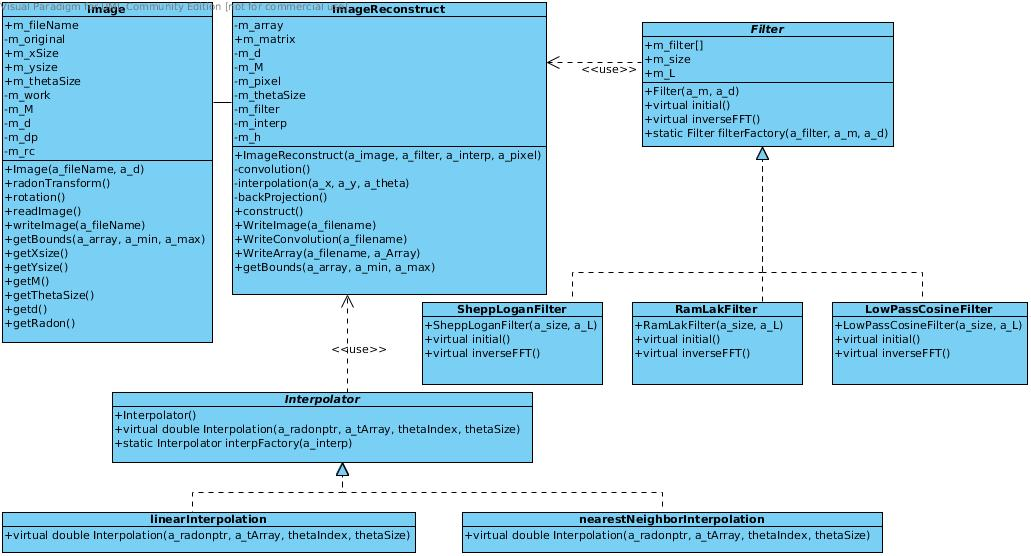
\includegraphics[width=490pt]{Figures/cd.jpg}
	\caption[Class diagram.]{Class diagram.}
	\label{fig:cd}
\end{figure}
\section{Implementation Approach}
C++ programming language in UBUNTU 12.04 platform with g++ 4.6 compiler was used to accomplish this software product. Factory design pattern was used to implement different interpolators and filters that derived from the base class. The idea of the factory pattern is to have the classes ability to create other classes without them knowing about all the possible classes that exists. 

\section{A Top Level Design of the Software}
Image reconstruction algorithm (\ref{algo}) is implemented using two main classes, i.e. \textit{Image} and \textit{ImageReconstruct} and another few minor classes for filters and interpolations. A top level design of the software used to solve this problem in the form of header files is given below.
\subsection{Image Class}
Main task of this class is to read the phantom image and compute the corresponding Radon transform. The constructor takes the file name of the image in order to read it into a RectMDArray m\_original. The double number a\_d is stored in the member data m\_d which gives the beam spacing for radon transformation. The results of the radon transformation will be updated into the member data m\_work with the type of RectMDArray which will be used in the ImageReconstruct class. This class also provides a method to write out the result of Radon transformation for testing purpose.  

\begin{verbatim}
class Image
{
public:
  Image(std::string a_fileName, double a_d);
  void radonTransform();
  void WriteImage(std::string a_fileName);
  void getBounds(RectMDArray<double>& a_array,double & a_min, double & a_max);
  int getXsize() {return m_xsize;}
  int getYsize() {return m_ysize;}
  int getM() {return m_M;}
  int getThetaSize() {return m_thetaSize;}
  double getd() {return m_d;}
  double gethalfLen() {return m_rc;}
  RectMDArray<double> getRadon() {return m_work;}
  std::string m_fileName; // Record the name of phantom image file.
 private:
  RectMDArray<double> m_original;
  RectMDArray<double> m_work;
  int m_xsize; // Record the size in the x direction of the matrix data.
  int m_ysize; // Record the sizx in the y direction of the matrix data.
  int m_thetaSize;// Record the number of rotations for the image.
  int m_M; // Record the half number of beams except zero position beam.
  double m_d; // Record the beam spacing in units
  double m_dp; // Record the beam spacing in pixels
  double m_rc; // Record the center of the image along diagonal
};
\end{verbatim}

\subsection{ImageReconstruct Class}
This class is the core of the design, which provides the major functionalities such as convolution and back projection. The member data m\_array is used to store the result of radon transformation from the Image class and after the call of convolution it will be updated to store the results of convolution. The constructor will take Image object as an input and also two integer which indicates the choices of the specific filter and interpolator. Based on the choice given by the user, the constructor will call the two static factory function of the Filter class and Interpolator class to generate the pointer to the specific derived class. The destructor of ImageReconstruct class is used to delete the filter and Interpolator pointer since these two are generated by new. Inverse FFT of the filter class are invoked inside the convolution function while interpolation functions are called inside the back projection function.   
\begin{verbatim}
class ImageReconstruct
{
public:
  RectMDArray<double> m_matrix;
  ImageReconstruct(Image & a_image, int a_filter, int a_interp, int a_pixel);
  ~ImageReconstruct();
  void construct();
  void WriteImage(std::string a_fileName);
  void WriteConvolution(std::string a_fileName);
  void WriteArray(std::string a_fileName, RectMDArray<double> a_Array);
  void getBounds(RectMDArray<double>& a_array,double & a_min, double & a_max);
 
private:
  void convolution(); // find the filtered radon transform
  void backProjection(); 
  RectMDArray<double> m_array;
  double m_d; // separation between neighbor beams
  int m_M;
  int m_thetaSize;
  int m_pixel;
  double m_h; // grid spacing in final grid
  Filter * m_filterptr;
  Interpolator * m_interpptr;
};
\end{verbatim}

\subsection{Interpolator Class}
This class is a base class which has two virtual functions that are implemented inside the derived classes shown below. In order to let user implement different Interpolation in the image reconstrcution class a factory function method is used for this base class. The factory function takes one integer indicating a specific Interpolator to create a pointer to the derived class and it returns a pointer to base class.
\begin{verbatim}
class Interpolator
{
public:
  Interpolator(){};
  virtual ~Interpolator(){};
  virtual double Interpolation(double * a_radonptr, vector<double> & a_tArray, 
      double a_t, int thetaIndex, int thetaSize) const =0;
  static Interpolator * interpFactory(int a_interp);
};  
\end{verbatim}

\paragraph{LinearInterpolator Class.}
This is a one of the derived classes of the Interpolator class, which provides the linear interpolation functionality by implementing the inherited virtual Interpolation function.  
\begin{verbatim}
class linearInterpolator:public Interpolator
{
public:
  double Interpolation(double * a_radonptr, vector<double> & a_tArray, 
  double a_t, int thetaIndex, int thetaSize) const;
};
\end{verbatim}

\paragraph{NearestNeighborInterpolator Class.}
This is the other derived class of the Interpolator class, which provides the nearest neighbor interpolation functionality by implementing the inherited virtual Interpolation function.  
\begin{verbatim}
class nearestNeighborInterpolator: public Interpolator
{
public:
  double Interpolation(double * a_radonptr, vector<double> & a_tArray, double a_t, int thetaIndex, int thetaSize) const;
};
\end{verbatim}

\subsection{Filter Class}
This class is a base class which has three virtual functions that are implemented inside the derived classes shown below. The factory function filterFactory is also used here.
\begin{verbatim}
class Filter
{
public:
  Filter(int a_m, double a_d){ m_size=2*a_m; m_L = 1.0/(2.*a_d); m_filter.resize(2*m_size+1); } 
  virtual ~Filter(){};
  virtual void inverseFFT()=0; 
  virtual void initial() = 0;
  static Filter* filterFactory(int a_filter, int a_m, double a_d);
  vector<double> m_filter;
  int m_size; // the size of filter = 2*m_size +1 = 4*a_size +1
  int m_L;
};  
\end{verbatim}

\paragraph{SheppLoganFilter Class.}
This is a one of the derived classes of the Filter class, which provides the Shepp-Logan filter functionality by implementing the inherited virtual inversFFT function.  
\begin{verbatim}
class SheppLoganFilter: public Filter
{
public:
  SheppLoganFilter(int a_size, double a_L): Filter(a_size, a_L) { }; 
  void inverseFFT(){};
  void initial(){};
};
\end{verbatim}

\paragraph{RamLakFilter Class.}
This is a another derived class of the Filter class, which provides the Ram-Lak filter functionality by implementing the inherited virtual inversFFT function.  
\begin{verbatim}
class RamLakFilter: public Filter
{
public:
  RamLakFilter(int a_size, double a_L): Filter(a_size, a_L) { }; 
 void inverseFFT(){};
 void initial(){};
};
\end{verbatim}

\paragraph{LowPassCosineFilter Class.}
This is also a derived classes of the Filter class, which provides the low-pass cosine filter functionality by implementing the inherited virtual inversFFT function.  
\begin{verbatim}
class LowPassCosineFilter: public Filter
{
public:
  LowPassCosineFilter(int a_size, double a_d): Filter(a_size, a_d) { };
  void inverseFFT(){};
  void initial(){};
};
\end{verbatim}



